\chapter{結論}
\label{conclusion}

本章では、本論文のまとめと今後の展望を示す。

\section{本研究のまとめ}

本研究では、インターネット上の複数の拠点に同一のLayer 2ネットワークを拡張することができる一対多型のLayer 2ネットワーク
拡張技術であるLEONの設計と実装をした。現在のインターネットには、宛先と直接通信した場合より、他の拠点を経由して宛先と通信
した場合の方が、通信をする際の遅延が小さくなる場合がある。LEONはトンネル終端点間の遅延を計測し、その計測結果をもとに遅延が最も
遅延が小さくなる経路を計算する。これにより、LEONを利用することにより、イーサネットフレームを遅延の最も小さい経路で転送できるようになった。
その結果、本研究で行った実験から、LEONを利用して拡張されたLayer 2ネットワーク上で通信を行った場合、従来手法と比べ、
サービスを構成するコンポーネントのパフォーマンスが改善され、サービスのパフォーマンスも改善されるということがわかった。
しかし、LEONでは全てのトンネル終端点が他のトンネル終端点の状態管理や遅延計測などを行う必要があるため、
トンネル終端点が増加することによりトンネル終端点の負荷が高くなるため様々な悪影響が生じる。
本研究で行った実験から、トンネル終端点の増加が与える影響の1つとして、中継を行なっているトンネル終端点での障害発生から、そのトンネル終端点を経由していた通信が再び可能になるまで
かかる時間の増加があるということがわかった。そのため、LEONは多くの拠点にLayer 2ネットワークを拡張するには適していない
ということもわかった。

\section{今後の展望}

本研究で提案したLayer 2ネットワーク拡張技術であるLEONは、中継を行なっているトンネル終端点で障害が発生してから、
再びそのトンネル終端点を中継して行われていた通信が行えるようになるまで、最大で120秒かかる。そのため、最大120秒間、通信が行えない
間に、送信されたイーサネットフレームがパケットロスされてしまう可能性やサーバーから切断されてしまうなどといった
問題の原因となることが想定される。また、図~\ref{img:tenbou1}で示すように、ファイアーウォールの設定や拠点間のネットワーク
障害などにより、直接通信することはできないが、他のトンネル終端点からは到達することができる場合が考えられる。LEONは
このよう場合、直接通信することができないトンネル終端点は障害発生と判断し、トンネル終端点リストから消去してしまう。
そのため、Layer 2ネットワークが分断してしまうという問題がある。これらの問題を解決するためには、より優れた障害検知
の手法が必要である。

\begin{figure}
	\begin{center}
		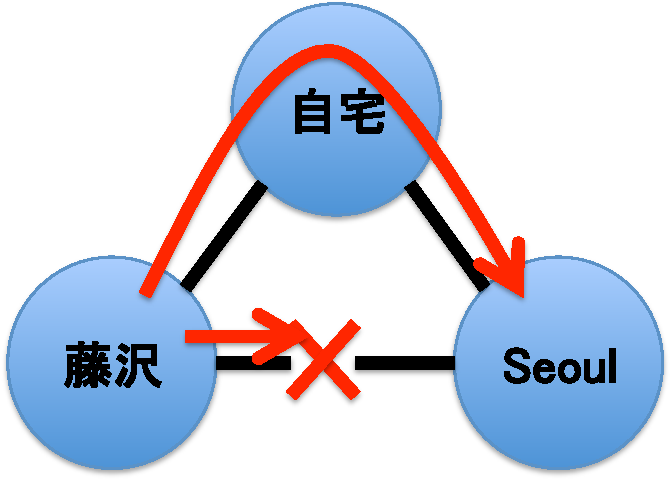
\includegraphics[scale=0.60]{./img/tenbou1}
		\caption{直接通信をすることができない状況}
		\label{img:tenbou1}
	\end{center}
\end{figure}

また、本研究で提案した手法は、トンネル終端点間の遅延を計測し、その計測結果をもとに経路の計算を行った。しかし、インターネット
には遅延は小さいが帯域幅は細いトンネル終端点や、遅延は大きいが帯域幅は太いトンネル終端点が存在する可能性がある。WIDE Cloudの
ように拡張されたLayer 2ネットワーク上で様々なアプリケーションが動作するような環境では、遅延よりも帯域幅を優先したほうがパフォーマンス
が高くなるアプリケーションも動作している可能性がある。そのため、Layer 2ネットワーク拡張技術はトンネル終端点間の遅延だけでなく、Layer 2ネットワーク上
で動作するアプリケーションやトンネル終端点間の帯域幅も考慮する必要がある。

%%% Local Variables:
%%% mode: japanese-latex
%%% TeX-master: "../yummy_bthesis"
%%% End:
